% !TEX root =  paper.tex
\section{Introduction}

\begin{figure}[t]
	\subfloat[]{
	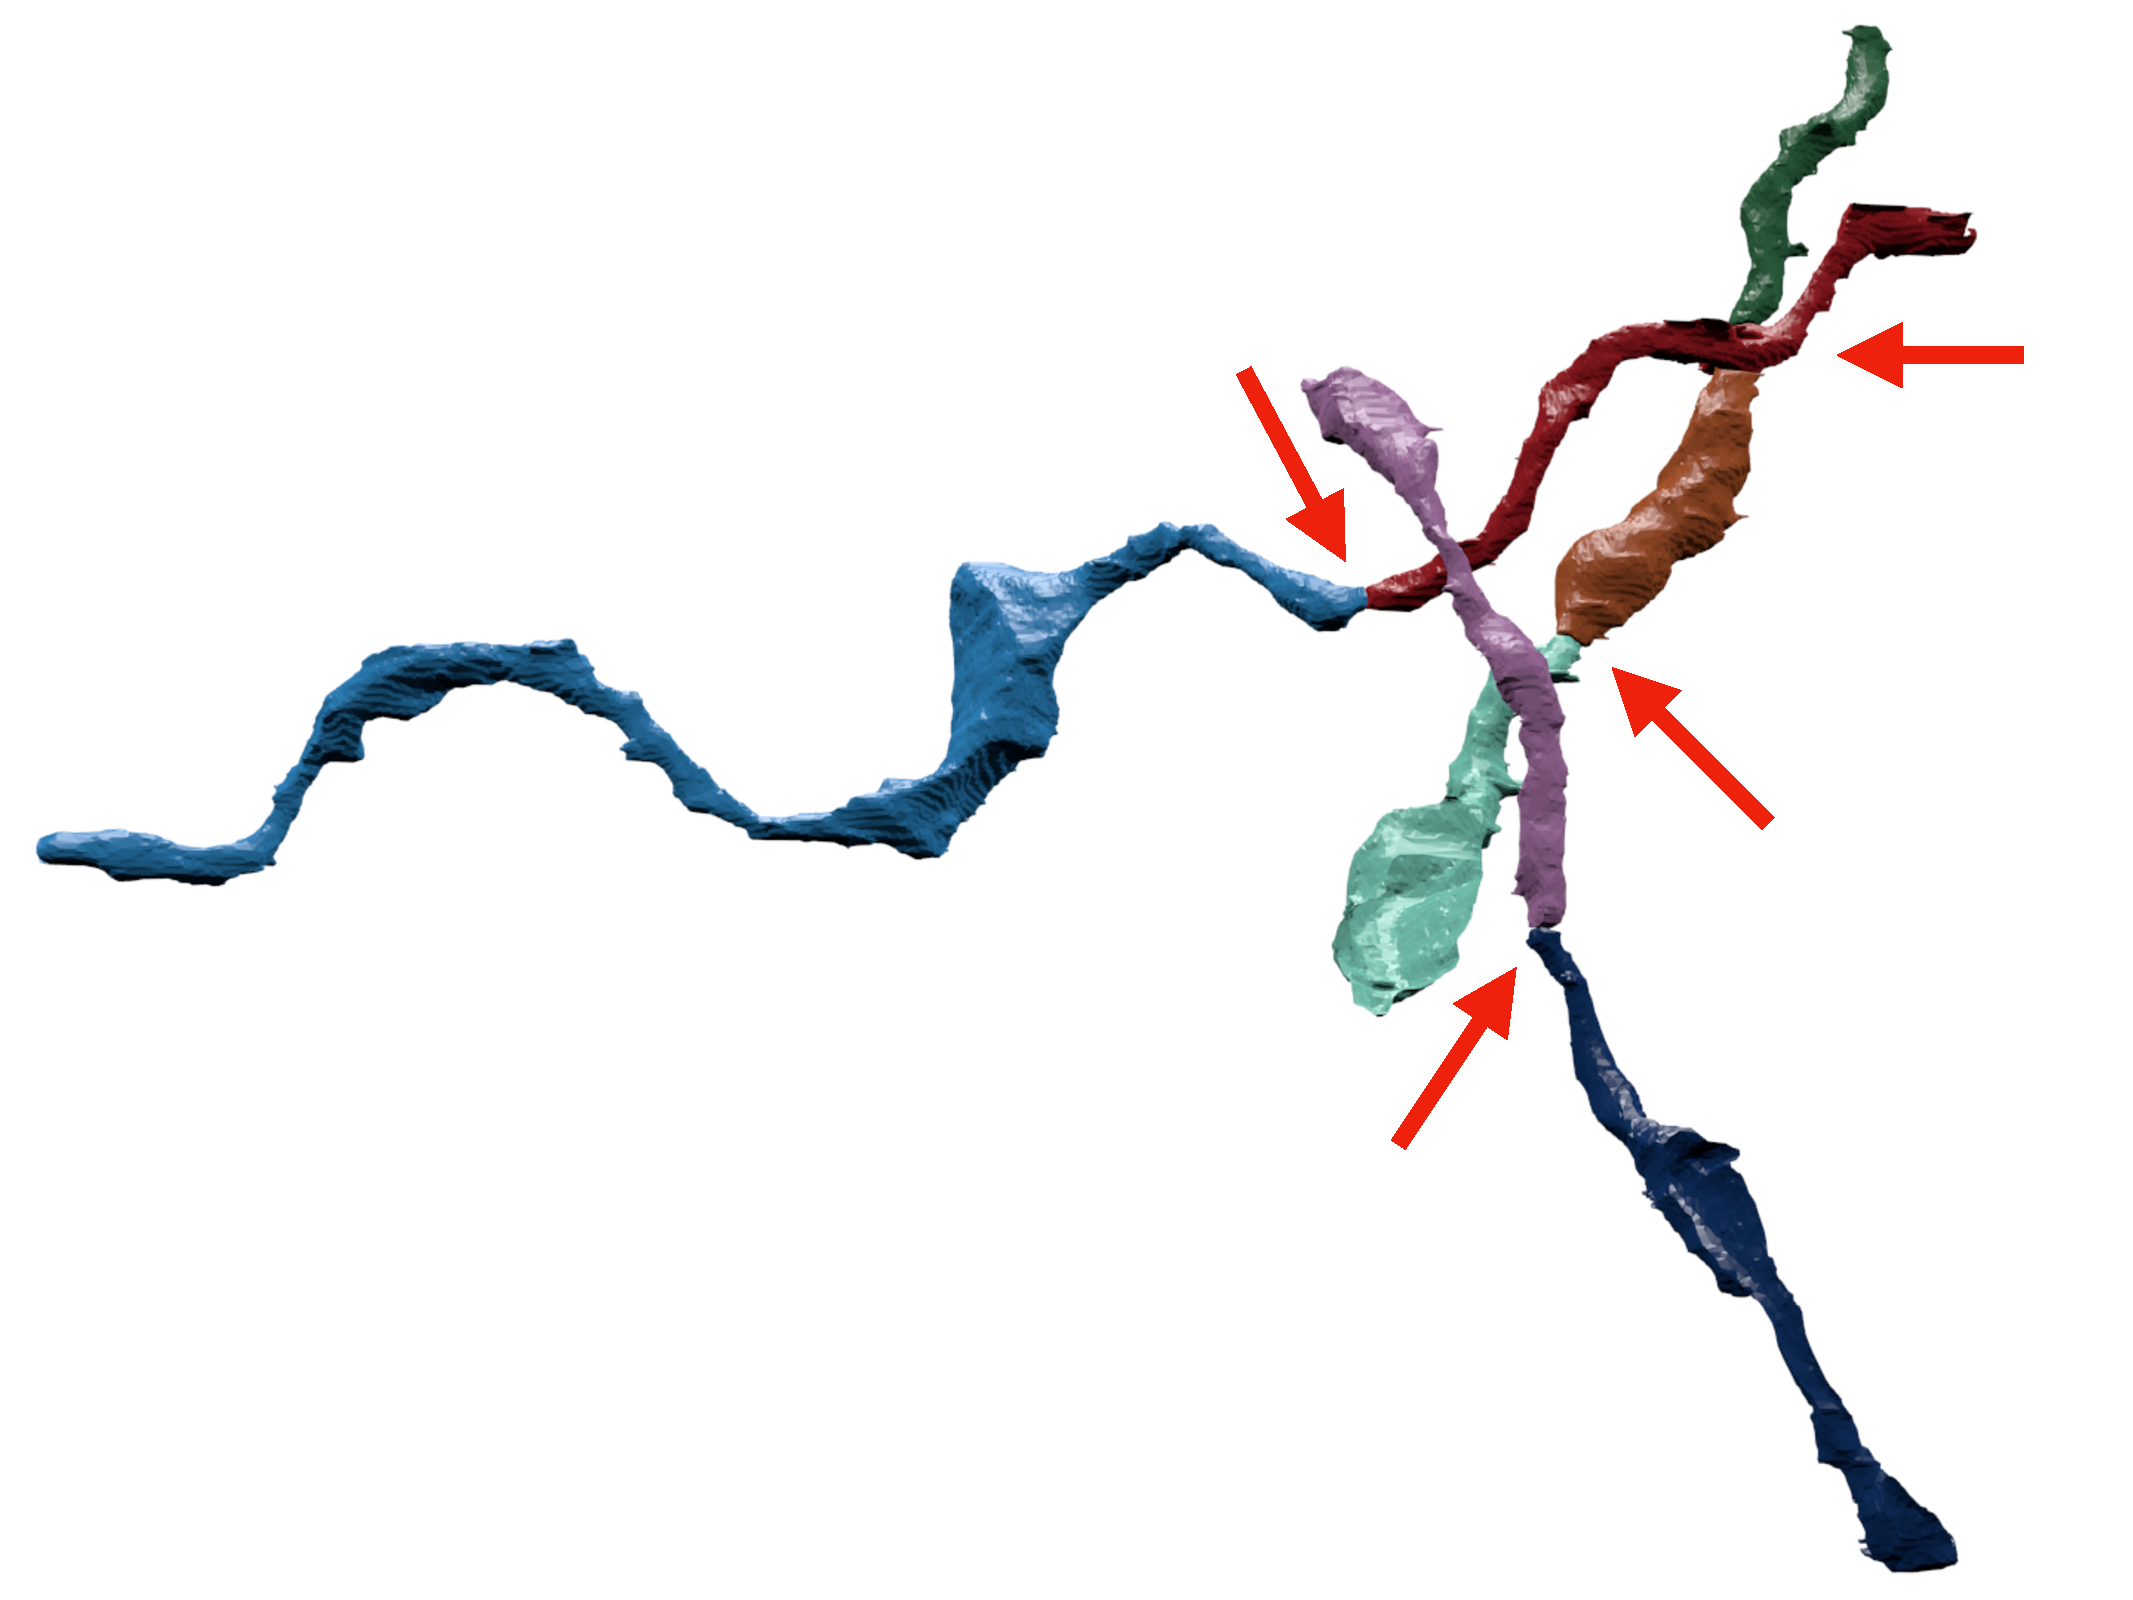
\includegraphics[width=.47\linewidth]{figures/schema/pre-multicut-with-arrows.pdf}
	}
	\subfloat[]{
	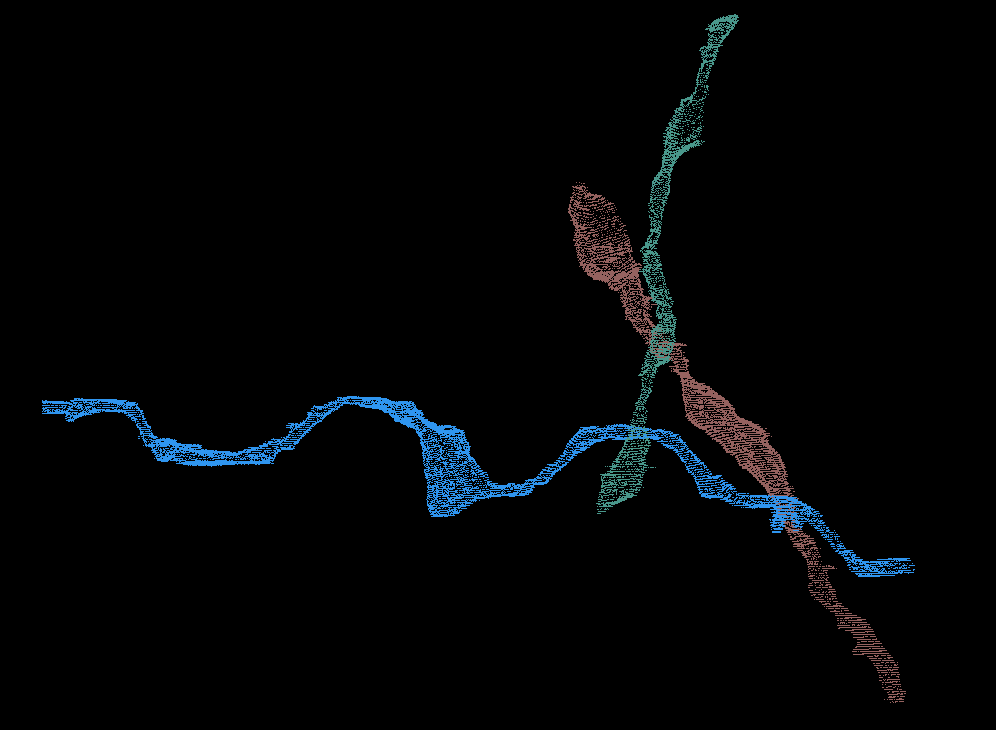
\includegraphics[width=.47\linewidth]{figures/schema/post-multicut.png}
	}
	\caption{Example improvement of neural reconstruction. (a) We extract 3D skeletons from pixel-based segmentation algorithms to create a 3D graph representation. Edges with high segmentation error probabilities are indicated by the red arrows. (b) We improve the accuracy of segmentation  using a graph partitioning algorithm, leveraging both local and global information.}
	\label{fig:teaser}
\end{figure}

%\donglai{usually, top-down means split.. but we are also bottom-up, but with different representation}
The field of connectomics is concerned with reconstructing the wiring diagram of the brain at nanometer resolutions to enable new insights into the workings of the brain~\cite{haehn2017scalable,kasthuri2015saturated}. Recent advancements in image acquisition using multi-beam serial-section electron microscopy (sSEM) have allowed researchers to produce terabytes of image data every hour~\cite{hildebrand2017whole}. It is not feasible for domain experts to manually reconstruct this vast amount of image data~\cite{haehn2014design}. State-of-the-art automatic reconstruction approaches use pixel-based segmentation with convolutional neural networks (CNNs) followed by agglomeration strategies~\cite{seymour2016rhoananet,lee2015recursive,nunez2014graph,parag2017anisotropic,ronneberger2015u,zlateski2015image}.
These \textit{bottom-up pixel-based} methods produce excellent results but still fall short of acceptable error rates for large volumes.

\begin{figure*}[t]
	\centering
	\subfloat[]{
	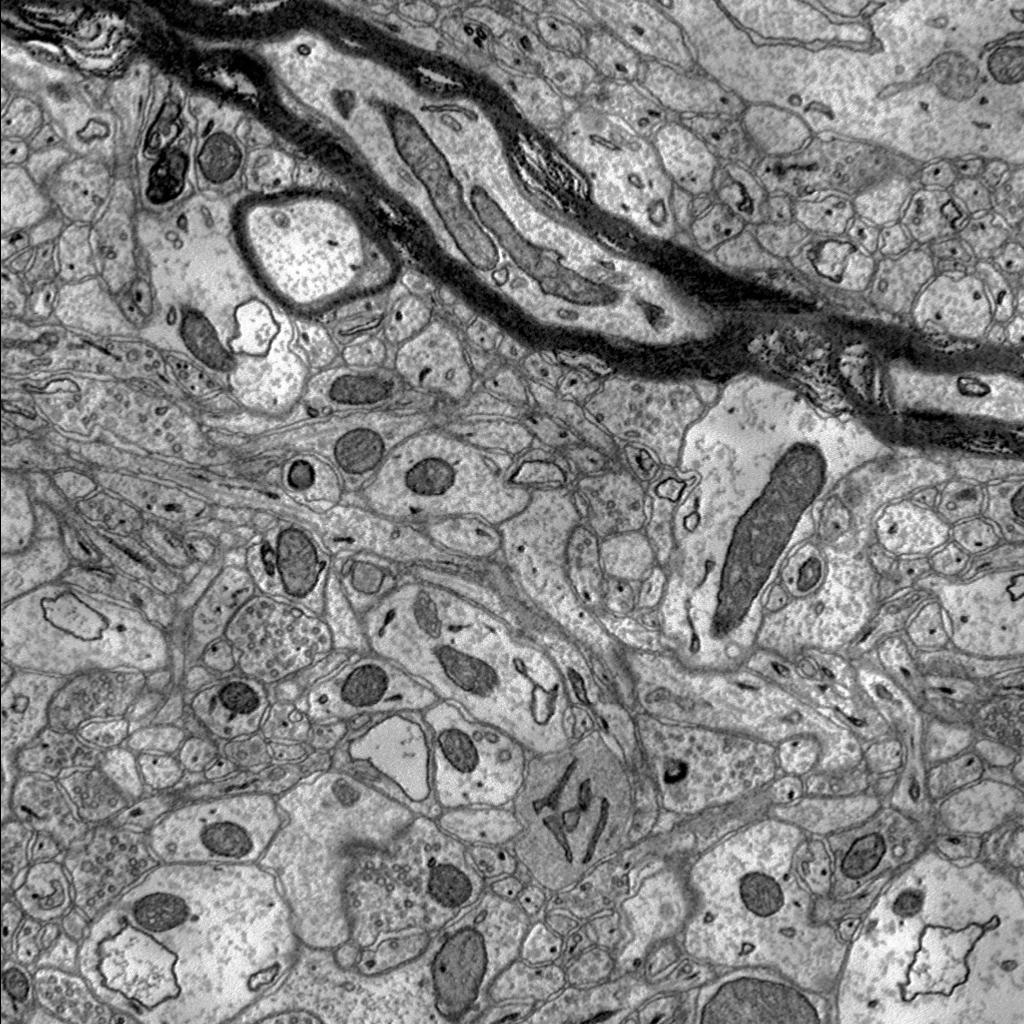
\includegraphics[width=.24\linewidth]{./figures/pipeline/image.png}
	}
	\subfloat[]{
	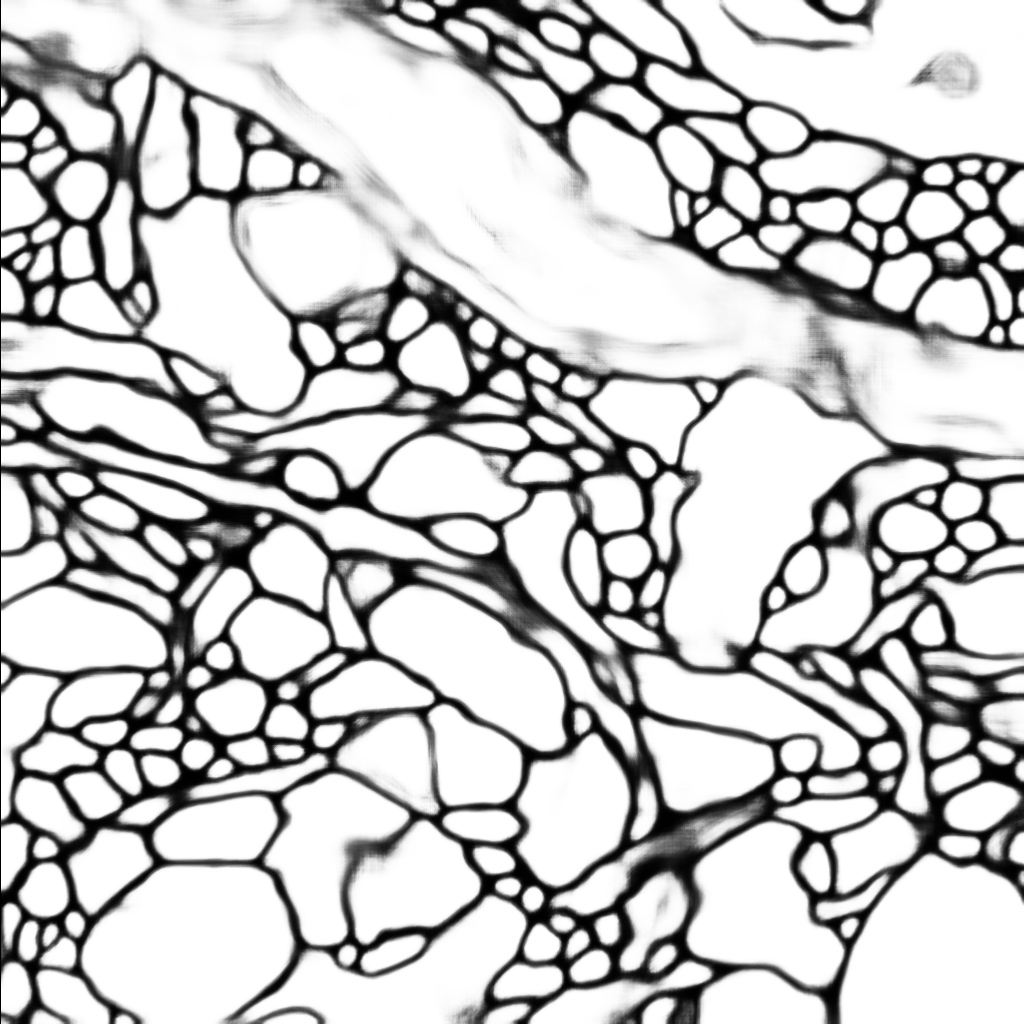
\includegraphics[width=.24\linewidth]{./figures/pipeline/affinities.png}
	}
	\subfloat[]{
	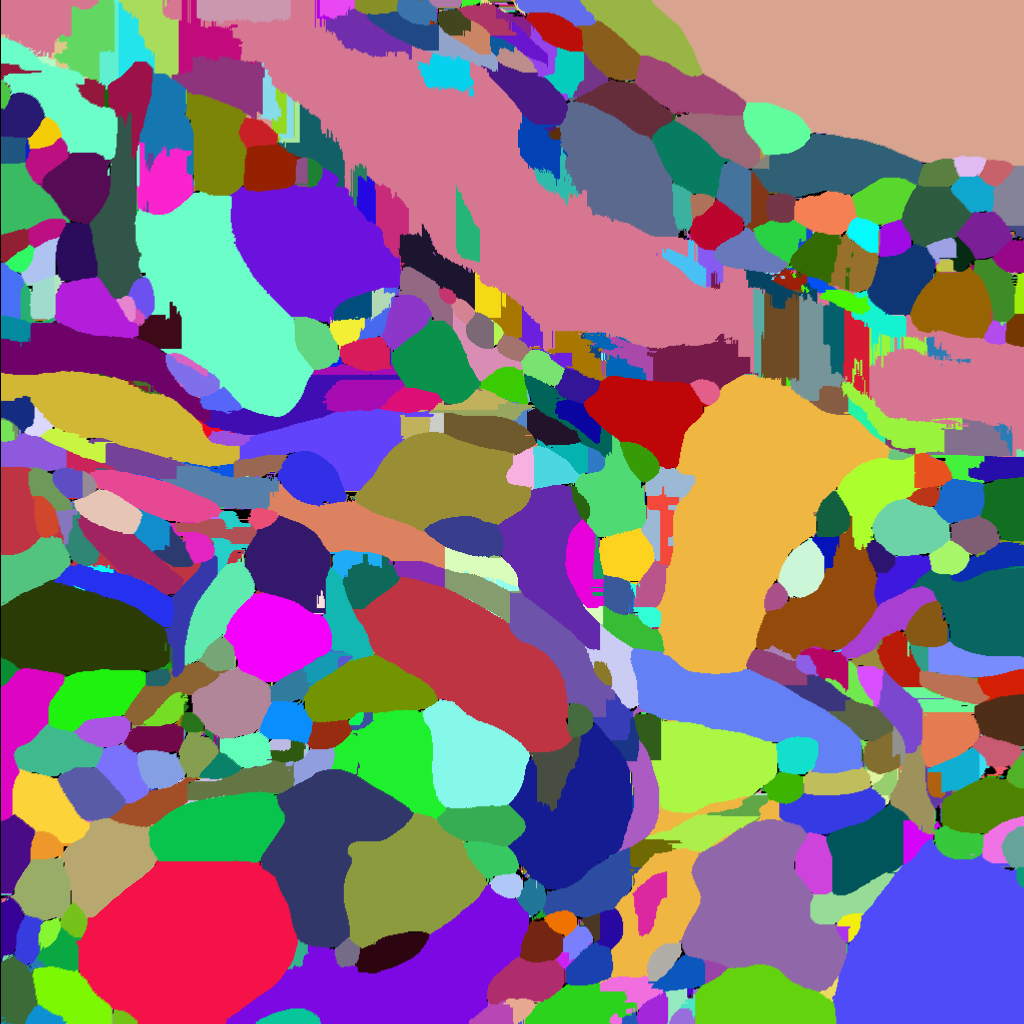
\includegraphics[width=.24\linewidth]{./figures/pipeline/watershed.png}
	}
	\subfloat[]{
	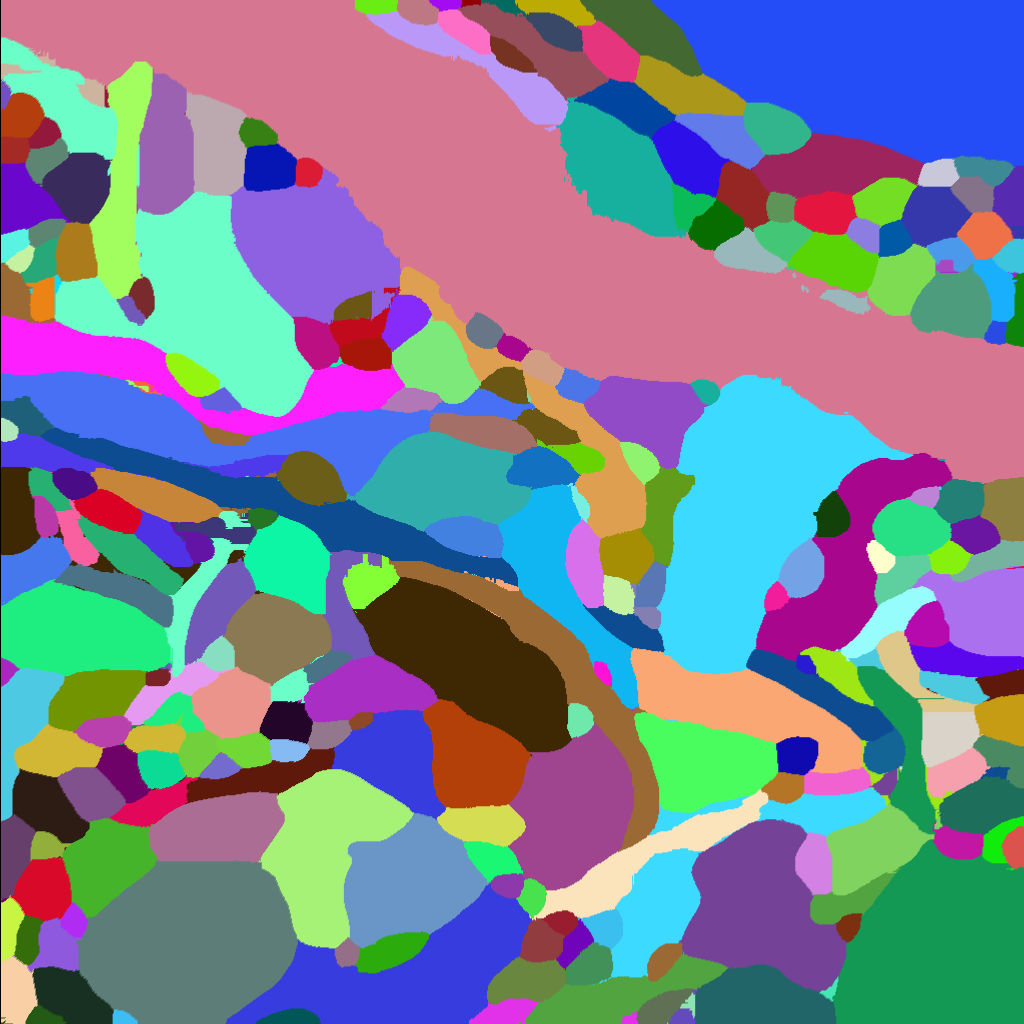
\includegraphics[width=.24\linewidth]{./figures/pipeline/neuroproof.png}
	}
	\caption{An overview of a pixel-based connectomics segmentation pipeline. (a) Original EM image data (b) Output of a CNN predicting voxel affinities (c) Clustering of the affinities using a watershed algorithm (d) Agglomeration of the super-voxels into larger segments.}
	\label{fig:pipeline}
\end{figure*}

%
%\begin{figure*}[t!]
%	\centering
%	(a) 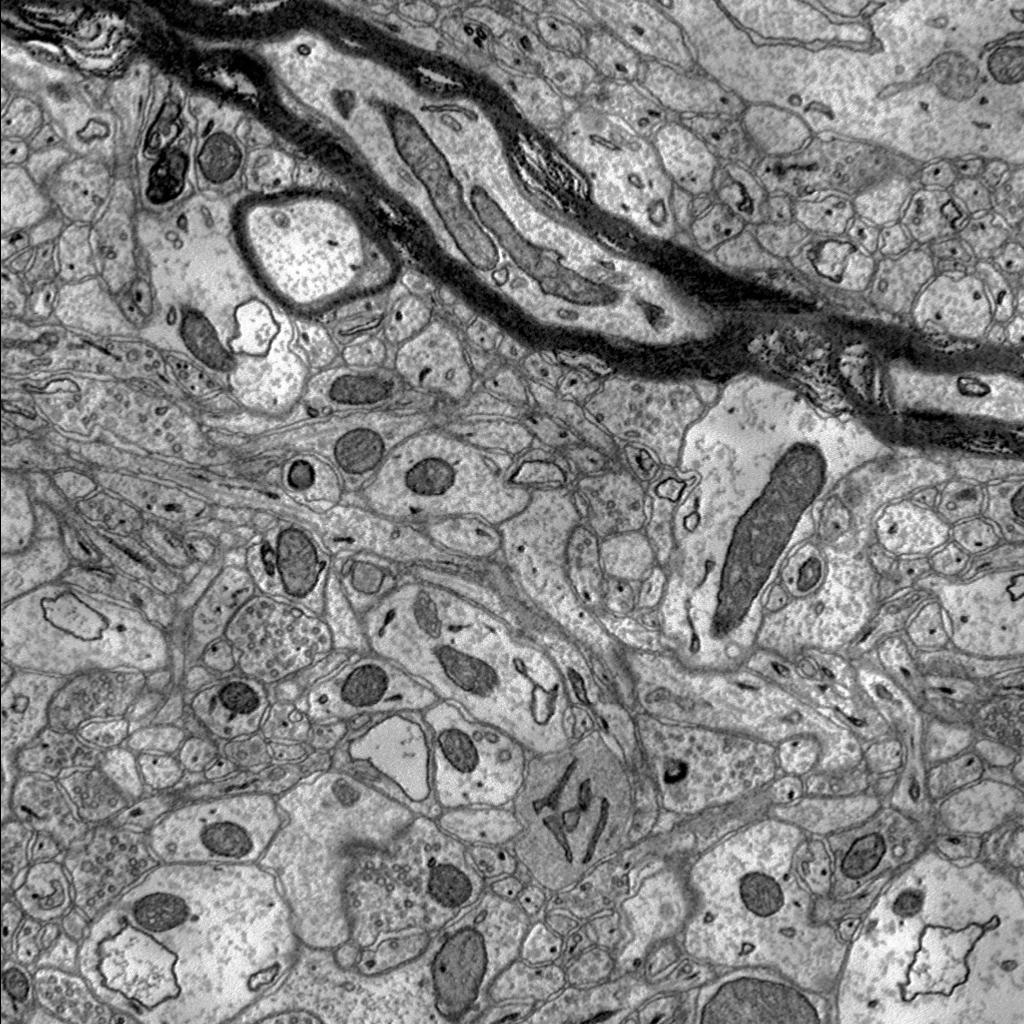
\includegraphics[width=0.18\linewidth]{./figures/pipeline/image.png}
%	\hspace{0.025\linewidth}
%	(b) 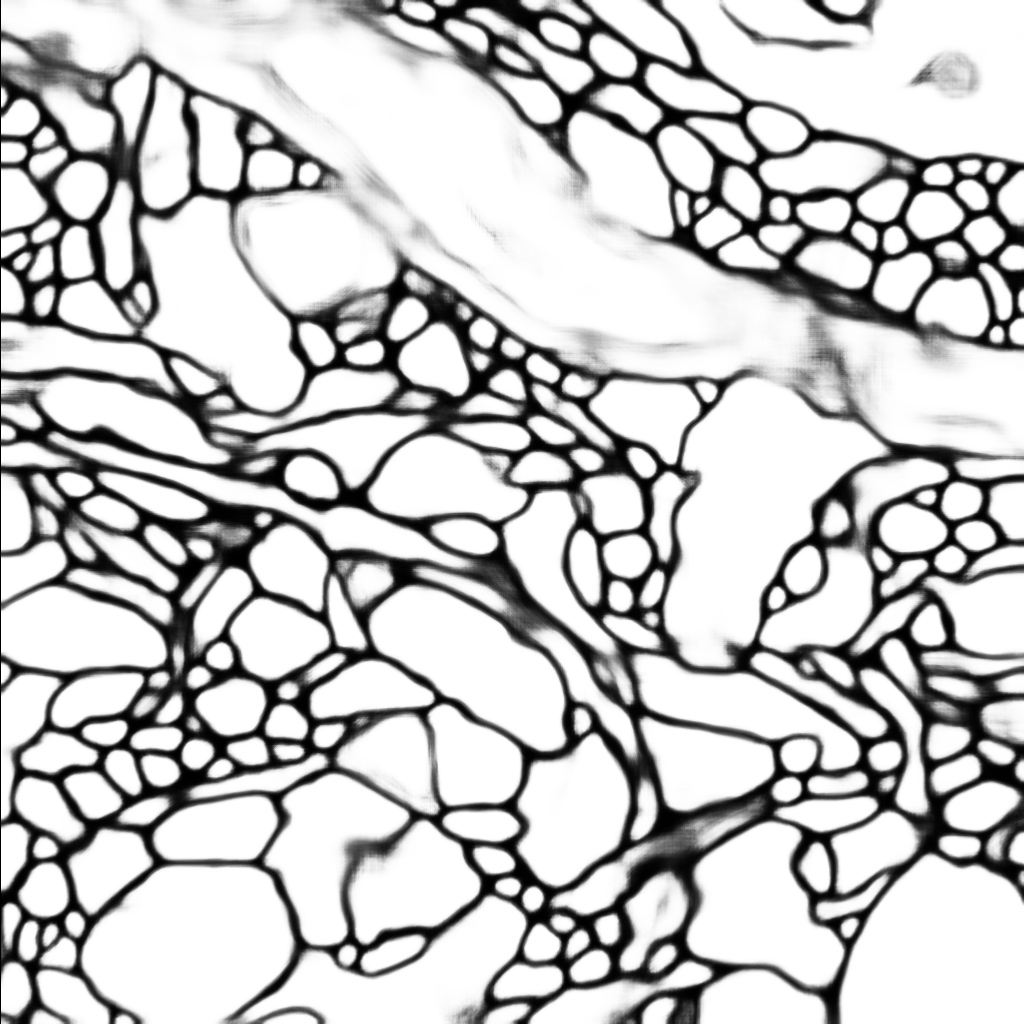
\includegraphics[width=0.18\linewidth]{./figures/pipeline/affinities.png}
%	\hspace{0.025\linewidth}
%	(c) 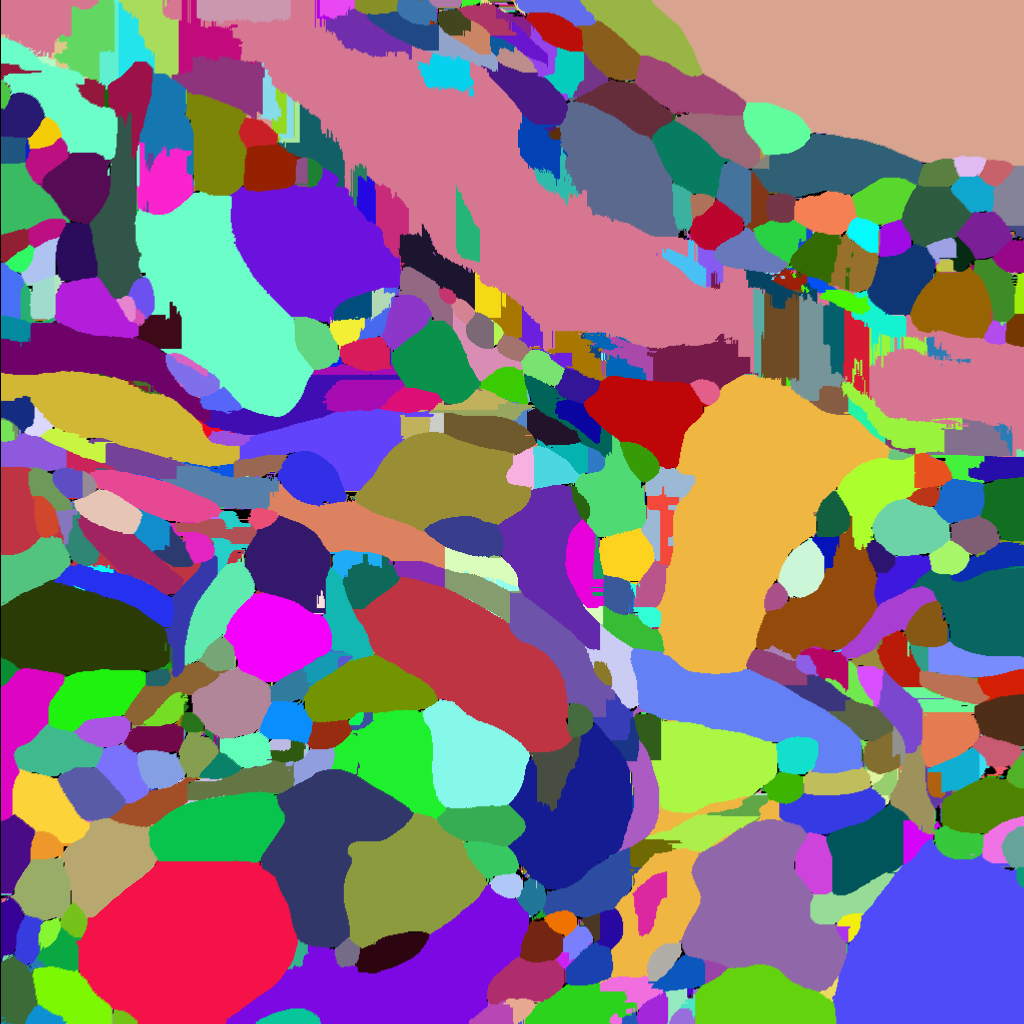
\includegraphics[width=0.18\linewidth]{./figures/pipeline/watershed.png}
%	\hspace{0.025\linewidth}
%	(d) 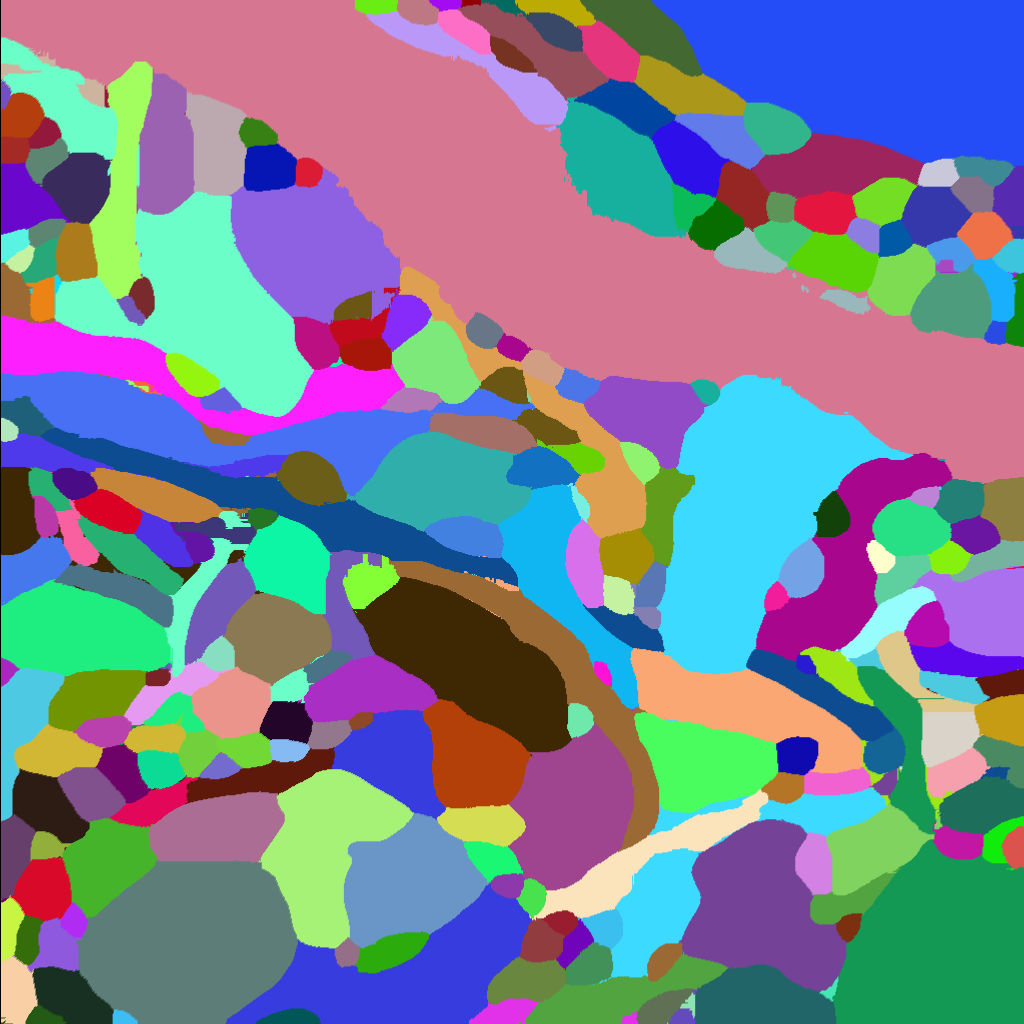
\includegraphics[width=0.18\linewidth]{./figures/pipeline/neuroproof.png}
%	\caption{An overview of a pixel-based connectomics segmentation pipeline. (a) Original EM image data (b) Output of a CNN predicting voxel affinities (c) Clustering of the affinities using a watershed algorithm (d) Agglomeration of the super-voxels into larger segments.}
%	\label{fig:pipeline}
%\end{figure*}
%
%Researchers address the failures of these pixel-based algorithms by training random-forest classifiers to agglomerate an oversegmentation of voxels~\cite{nunez2014graph,10.1371/journal.pone.0125825}.
%These classifiers take the output of the pixel-based algorithms as input and generate high-level statistics such as affinity distributions between regions.
%Presently, these methods use hand-designed features despite the evidence that machine-learned features perform better~\cite{bogovic2013learned}.
%These \textit{region-based} algorithms outperform the pixel-based algorithms but do not provide the accuracy needed for large scale reconstructions of the brain.

%Here we introduce a scalable, top-down segmentation algorithm that also leverages local information.
%Partitioning globally allows us to apply domain-specific constraints to the segmentation task.
%We extract a graph representation from the input segmentation.
%By simplifying the 3-D segments by their skeletons, we can quickly generate the graph nodes and edges.

We present a \textit{top-down graph-based} method that builds on the outputs of bottom-up pixel-based segmentation approaches. We first extract 3D skeleton networks from the input segmentation and generate a simplified 3D graph (Fig.~\ref{fig:teaser}a). We train a CNN classifier on the agglomerated regions in the segmentation data to detect errors. We run the classifier to populate the graph edge weights with error probabilities. We then use a graph optimization algorithm to partition the graph into the final improved reconstruction by enforcing domain-specific global constraints from biology (Fig.~\ref{fig:teaser}b).

Our approach operates at a level of abstraction above existing pixel-based methods. This allows us to leverage both local and global information to produce more accurate reconstructions. Our method is independent of image resolution and acquisition parameters, enabling its application to isotropic and anisotropic image data without retraining. Using the 3D graph induced by the segmentation allows us to enforce global biological constraints on the reconstruction. Our dual approach of assessing local decisions in a global context yields accuracy improvements over existing reconstruction methods.

This work makes the following contributions: (1) a novel top-down method using  graphs from skeletonized 3D networks for improved neural reconstruction of connectomics data; (2) a region-based CNN classifier to detect errors using the 3D graph as global constraint; (3) an empirical evaluation of our method on several connectomics datasets; (4) our method yields improved performance over a state-of-the-art pixel-based reconstruction approach on average by \FIX{X} percent without drastically increasing the running time.
